\section{Method}
\label{sec:method}

\begin{figure}[ht]
\centering
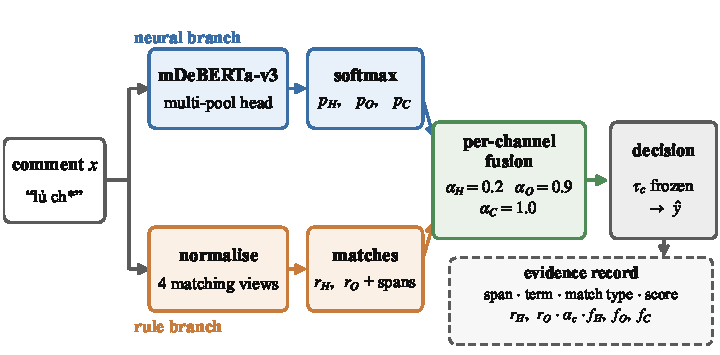
\includegraphics[width=0.80\textwidth]{figures/architecture.pdf}
\caption{The hybrid. A comment enters two branches: the neural branch produces class
probabilities, the rule branch per-label lexical scores and the spans that produced
them. Fusion mixes each channel with its own weight $\alpha_c$, and frozen per-channel
thresholds turn the three scores into a label; the evidence record is emitted with the
decision. Weights and thresholds shown were selected on validation for the focused
backbone.}
\label{fig:architecture}
\end{figure}

The hybrid has three parts: a rule engine that produces lexical scores and spans, a
transformer that produces class probabilities, and a fusion layer that combines them
channel by channel (Fig.~\ref{fig:architecture}). The branches share no parameters,
which allows the rule branch to be audited on its own.

\subsection{The lexical rule engine}
\label{sec:rule-engine}

\paragraph{Normalisation and views.}
The comment is Unicode-normalised to NFC, invisible characters removed, whitespace
collapsed, runs shortened to at most three, lower-cased while keeping diacritics. An
offset map reports a cleaned-view match as an original span. Auxiliary views handle
accent-less, leet, repeat-collapsed and separator-stripped (\texttt{n g u}) text.
Each hit records term, label, view, raw span and match type (e.g.\ \emph{exact},
\emph{accentless\_alias}, \emph{leet}, \emph{separator\_inserted}, \emph{fuzzy}).

\paragraph{Scoring.}
Every match $i$ receives
\begin{equation}
s_i \;=\; \sigma_{\ell(i)} \cdot c_i \cdot m_i \cdot \kappa_i ,
\label{eq:match}
\end{equation}
where $\sigma_{\ell(i)}$ is the severity of the matched label ($0.95$ for
\hate{}, $0.60$ for \off{} after tuning), $c_i$ the entry confidence from the
training split, $m_i$ the match-type factor and $\kappa_i$ a context factor for
quotation, negation and context-required terms. Matches of one label are
de-duplicated and aggregated with a saturating sum over at most $K=10$ matches:
\begin{equation}
r_\ell \;=\; 1-\prod_{i\in T_\ell}\left(1-s_i\right).
\label{eq:aggregate}
\end{equation}
For fusion they become a three-channel pseudo-probability
\begin{equation}
\tilde{\mathbf r} \;=\; \frac{1}{1+\min(r_H,r_O)}
\begin{bmatrix} r_H \\ r_O \\ 1-\max(r_H,r_O) \end{bmatrix},
\label{eq:pseudo}
\end{equation}
which preserves the ordering of the two toxic channels while placing \clean{} on
the same scale. When the rule is silent, $\tilde{\mathbf r}=(0,0,1)$: no evidence
is treated as maximal cleanliness evidence, an assumption
Sect.~\ref{sec:analysis} tests.

\paragraph{Tuning.}
Scoring weights are tuned on validation by greedy coordinate descent, thresholds
re-optimised per candidate; the test set is never loaded. The search made the engine more
aggressive (severity \hate{} $0.95$, accentless-alias $0.0$, repeat-collapsed $0.4$,
combined-obfuscation $0.3$, negation and context-required $1.0$): validation preferred
more matches over cautious ones.

\subsection{The neural branch}
\label{sec:neural}

We fine-tune \texttt{microsoft/mdeberta-v3-base}
\cite{he2023debertav3,liu2024mdeberta}. The focused backbone
(\model{sensitiveai-vi-custom}) uses a multi-pool head: \texttt{[CLS]}, mean and max
pooling concatenated, projected to a 512-dim bottleneck (dropout $0.1$), then three
logits. Training: cross-entropy, AdamW \cite{loshchilov2019adamw}, linear schedule
with 10\% warm-up, lr $3\times10^{-5}$, batch 16, max length 256, up to 30 epochs,
early stopping on validation macro-F1. Three further backbones share the encoder with
different recipes: standard head; two-stage with discriminative learning rates and
focal loss \cite{lin2017focal}; three-stage curriculum \cite{bengio2009curriculum}
with manual class weights.

\subsection{Fusion and decision}
\label{sec:fusion}

Let $p_c$ be the transformer probability for class $c$ and $\tilde r_c$ the
renormalised rule score. Per-channel fusion is
\begin{equation}
f_c \;=\; \alpha_c\,p_c \;+\; (1-\alpha_c)\,\tilde r_c,
\qquad c\in\{\hate{},\off{},\clean{}\}.
\label{eq:fusion}
\end{equation}
A single global $\alpha$ is the special case $\alpha_H=\alpha_O=\alpha_C$. A class
is \emph{accepted} when $f_c\ge\tau_c$; the accepted class with the highest $f_c$
wins, and if none is accepted the decision falls back to $\arg\max_c f_c$.

We compare four families: global $\alpha$ with argmax, global $\alpha$ with
thresholds, a multinomial logistic meta-classifier over six scores, and per-channel
$\alpha$ with thresholds, all selected on validation. The per-channel variant is primary:
classes have different rule behaviour (precise on \hate{}, weak on \off{}, uninformative
on \clean{}). Validation finds $\alpha_H=0.2$, $\alpha_O=0.9$, $\alpha_C=1.0$ and
$\tau_H=0.14$, $\tau_O=0.66$, $\tau_C=0.60$.

\subsection{Evidence record and protocol}
\label{sec:evidence}

For every comment the system emits, with the label, an evidence record: matched
raw-text spans, each span's term and label, matching view and match type, per-match
score, aggregated rule scores, per-channel weights and the three fused scores. Given
the record and the transformer probabilities, a reviewer can recompute the decision
exactly---our meaning of \emph{faithful by construction} for the lexical channel, while
the neural contribution remains a black box.
